\documentclass{article}
\usepackage{graphicx} % Required for inserting images
\usepackage[a4paper, total={6in, 8in}]{geometry}
\usepackage{subcaption}
\usepackage{float} % Required for positioning figures and tables at the specified location

\title{SC4003 Intelligent Agents Assignment 1}
\author{Amirul Hakim}
\date{\today}

\begin{document}

\maketitle

\section{Part 1 - Value Iteration and Policy Iteration}

\subsection{Method of value iteration}

\subsubsection{Description of Implemented Solution}

\paragraph{Initialization:} The environment is pass into the function by a class contains all the walls and rewards. A SummaryWriter object from tensorboardX is created for logging purposes. A utility values array V if initialized with zeros for each state in the environment.

\paragraph{Iteration:} The update step in the value iteration algorithm is:
\[V_{k+1}(s) = max_a \sum_{s'}P(s'|s, a) [R(s, a, s'), + \gamma V_k(s')] \]

where $V_k(s)$ is the utility of state $s$ at iteration $k$, $max_a$ denotes the maximum value over all possible actions $a$, $P(s' | s, a) $ is the probability of transitioning to state $s'$ from state $s$ to state $s'$ via action $a$, $\gamma$ is the discount factor which prioritizes immediate rewards over distant rewards, $V_k(s')$ is the utility of state $s'$ at iteration $k$.

Minimumly, it will run for 50 iterations while keep track of the maximum change in utility values $\delta$. Once it falls below a specified threshold, this indicates convergence

\paragraph{Plotting:} Plot the values and policies calculated from the above algorithm.

\subsubsection{Plot of Optimal Policy}

\begin{figure}[H]
    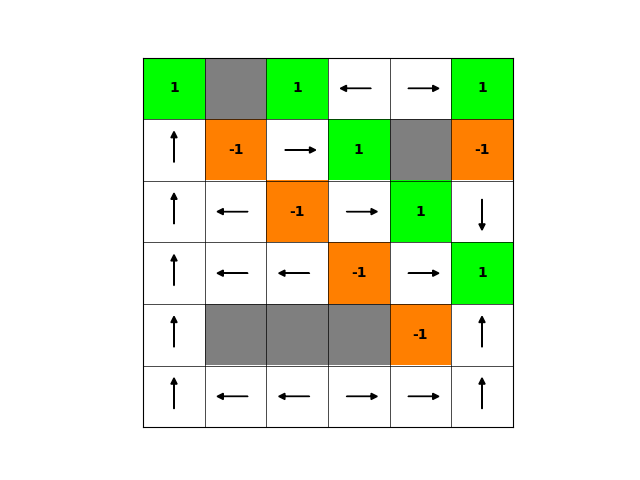
\includegraphics[width=100mm]{../asset/value_iteration_policy.png}
    \caption{The optimal policy for the gridworld is illustrated, where arrows indicate the recommended action in each state. The color of the arrows reflects the value associated with each action.}
    \label{fig:value_iteration_policy}
\end{figure}

\subsubsection{Utility of all states}

\begin{figure}[H]
    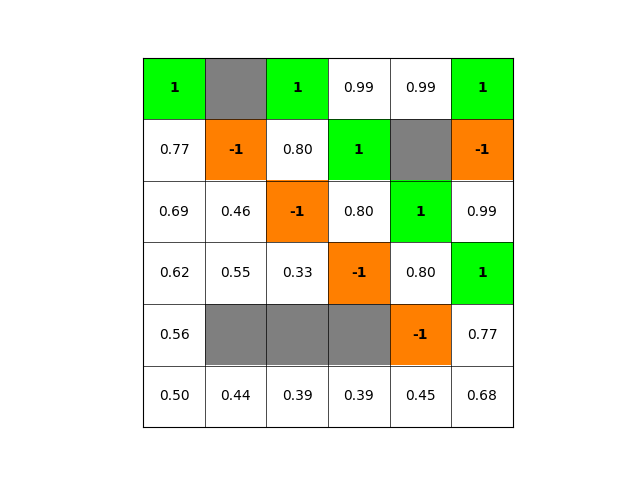
\includegraphics[width=100mm]{../asset/value_iteration_utility.png}
    \caption{The utility values of all states within the gridworld are shown, with the color of each cell representing the state's value.}
    \label{fig:value_iteration_utility}
\end{figure}

The more detailed value for the final utility is:

\begin{table}[H]
    \begin{tabular}{|l|l|l|l|l|l|}
        \hline
        0.0        & 0.0        & 0.0        & 0.99445061 & 0.98753071 & 0.0        \\\hline
        0.77247503 & 0.0        & 0.8        & 0.0        & 0.0        & 0.0        \\\hline
        0.68529708 & 0.4611854  & 0.0        & 0.8        & 0.0        & 0.99445061 \\\hline
        0.61840233 & 0.54986211 & 0.33239009 & 0.0        & 0.8        & 0.0        \\\hline
        0.56078941 & 0.0        & 0.0        & 0.0        & 0.0        & 0.77247503 \\\hline
        0.49686767 & 0.4406518  & 0.38504299 & 0.3947778  & 0.45040336 & 0.68411722 \\\hline
    \end{tabular}
\end{table}

\subsubsection{Convergence of value iteration}

\begin{figure}[H]
    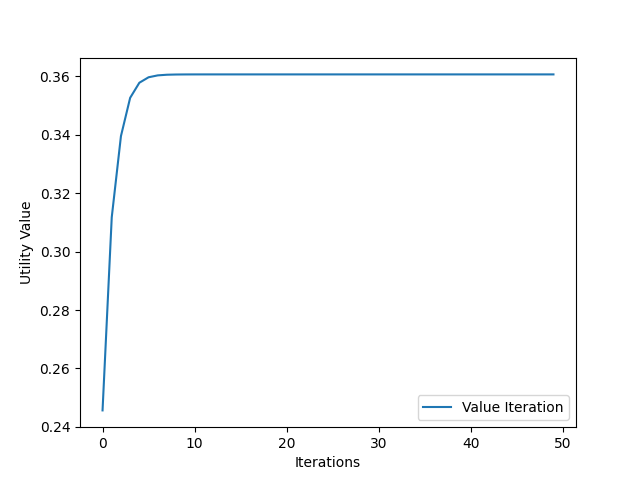
\includegraphics[width=100mm]{../asset/value_iteration_curve.png}
    \caption{Convergence of value iteration. The y-axis represents the maximum change in utility values across all states. The x-axis represents the number of iterations.}
    \label{fig:value_iteration_convergence}
\end{figure}

\subsection{Method of policy iteration}

\subsubsection{Description of Implemented Solution}

\paragraph{Initialization:} The setup is largely similar to value iteration, with the difference being that the initial policy assigns all actions to move right (0, 1).

\paragraph{Policy Evaluation:} For every state, the expected utility is calculated according to the current policy's action, taking into account the transition probabilities to all possible next states and their associated rewards.

\paragraph{Policy iteration:} The iteration consists of two steps: evaluation and improvement.

Policy Evaluation: 
\[V^\pi (s) = \sum_{s', r} P(s', r|s, \pi(s))[r + \gamma V^\pi (s')] \]

where $V^\pi(s)$ is the utility of state $s$ under policy $\pi$, $P(s', r | s, \pi(s))$ is the probability of transitioning to state $s'$ with reward $r$ from state $s$ when following policy $\pi$. $\gamma$ is the discount factor and $\pi(s)$ is the action prescribed by policy $\pi$ in state $s$.

Policy Improvement:
\[\pi ' (s) = arg max_a \sum_{s', r} P(s', r|s, a)[r + \gamma V^\pi (s')] \]

where $pi '(s)$ is the updated action for state $s$ under the improved policy $\pi '$, $argmax_a$ denotes the action that maximizes the expected utility.

\subsubsection{Plot of Optimal Policy}

\begin{figure}[H]
    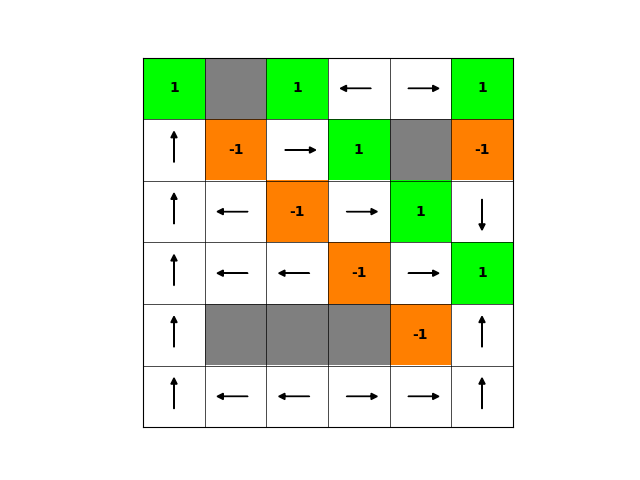
\includegraphics[width=100mm]{../asset/policy_iteration_policy.png}
    \caption{The optimal policy for the gridworld is illustrated, where arrows indicate the recommended action in each state. The color of the arrows reflects the value associated with each action.}
    \label{fig:policy_iteration_policy}
\end{figure}

\subsubsection{Utility of all states}

\begin{figure}[H]
    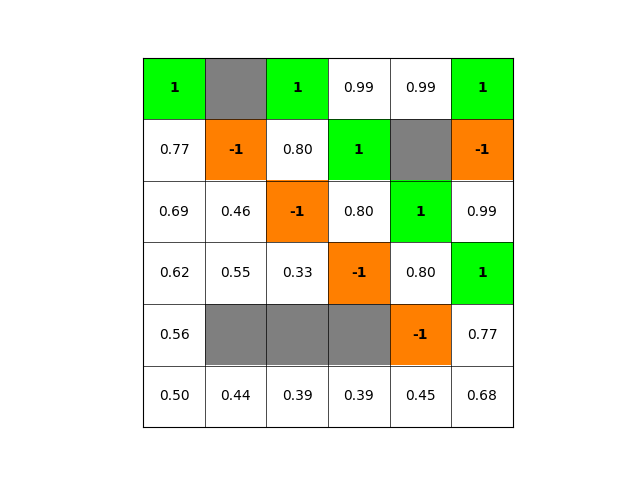
\includegraphics[width=100mm]{../asset/policy_iteration_utility.png}
    \caption{The utility values of all states within the gridworld are shown, with the color of each cell representing the state's value.}
    \label{fig:policy_iteration_utility}
\end{figure}

\begin{table}[H]
    \begin{tabular}{|l|l|l|l|l|l|}
        \hline
        0.0        & 0.0        & 0.0        & 0.99445061 & 0.98753071 & 0.0        \\\hline
        0.77247503 & 0.0        & 0.8        & 0.0        & 0.0        & 0.0        \\\hline
        0.68529708 & 0.4611854  & 0.0        & 0.8        & 0.0        & 0.99445061 \\\hline
        0.61840233 & 0.54986211 & 0.33239009 & 0.0        & 0.8        & 0.0        \\\hline
        0.56078941 & 0.0        & 0.0        & 0.0        & 0.0        & 0.77247503 \\\hline
        0.49686767 & 0.4406518  & 0.38504299 & 0.3947778  & 0.45040336 & 0.68411722 \\\hline
    \end{tabular}
\end{table}

This indicates that, under the default maze configuration, both policy iteration and value iteration converge to identical utility values.

\subsubsection{Convergence of policy iteration}

\begin{figure}[H]
    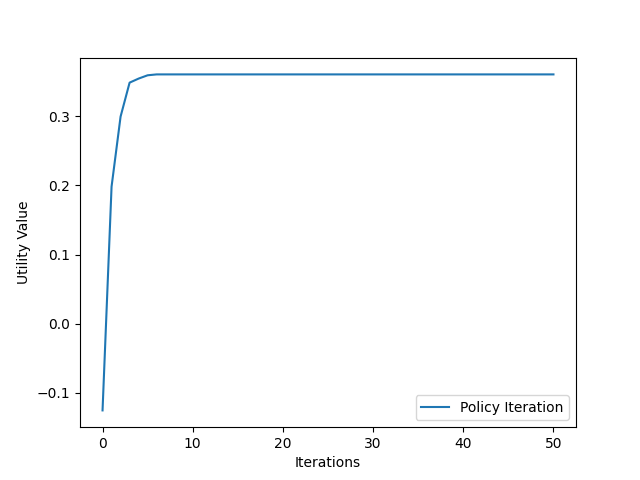
\includegraphics[width=100mm]{../asset/policy_iteration_curve.png}
    \caption{Convergence of policy iteration is illustrated, where the y-axis indicates the maximum change in utility values across all states, and the x-axis shows the number of iterations.}
    \label{fig:policy_iteration_convergence}
\end{figure}

\section{Part 2 - Complicated Maze Environment}

\subsection{Environment generation}

\paragraph{Randomly generated environment:} The environment is created by randomly distributing walls and rewards within the gridworld. The user specifies the number of walls and rewards. Both elements are placed at random locations in the environment. The resulting configuration is saved as a YAML file in the config folder. Below are examples of the generated environments:

\begin{figure}[H]
    \centering
    \begin{subfigure}{.5\textwidth}
        \centering
        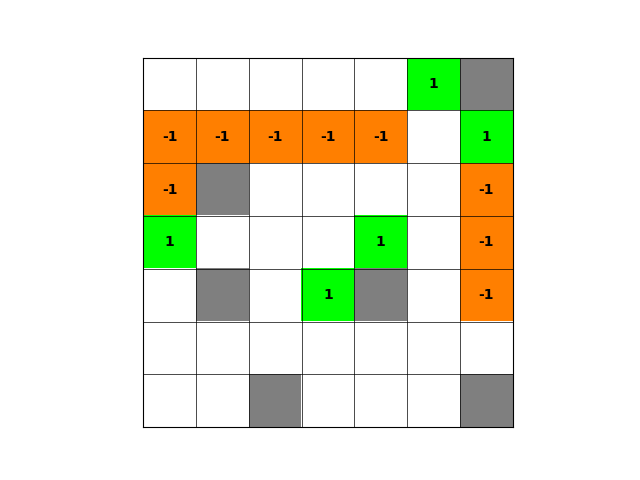
\includegraphics[width=60mm]{../results/maze_size_7/env.png}
        \caption{Maze size 7}
        \label{fig:random_env_1}
    \end{subfigure}%
    \begin{subfigure}{.5\textwidth}
        \centering
        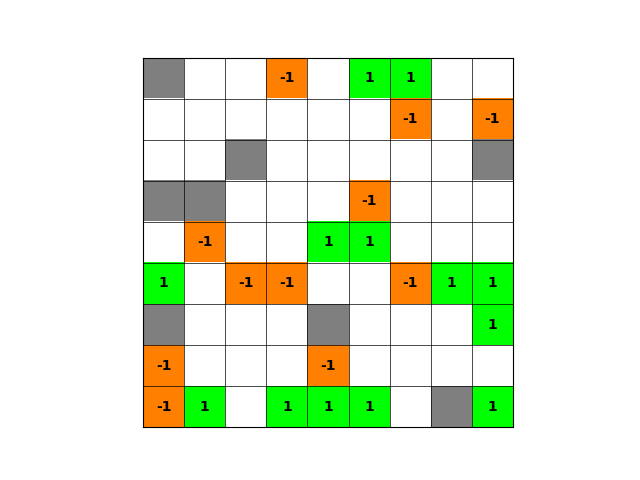
\includegraphics[width=60mm]{../results/maze_size_9/env.png}
        \caption{Maze size 9}
        \label{fig:random_env_2}
    \end{subfigure}
\end{figure}
\begin{figure}[H]
    \begin{subfigure}{.5\textwidth}
        \centering
        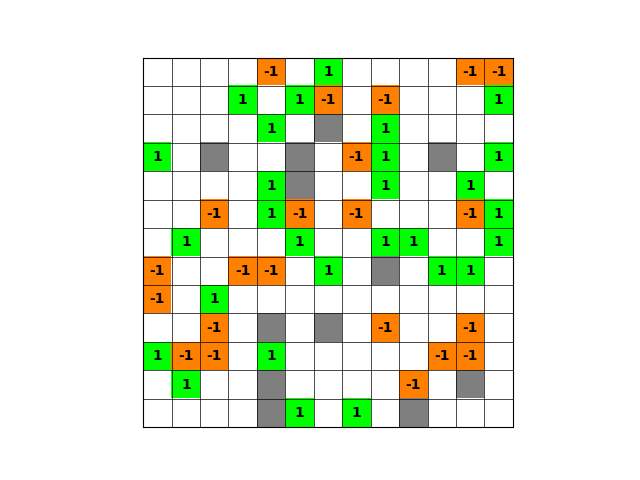
\includegraphics[width=60mm]{../results/maze_size_11/env.png}
        \caption{Maze size 11}
        \label{fig:random_env_3}
    \end{subfigure}
    \begin{subfigure}{.5\textwidth}
        \centering
        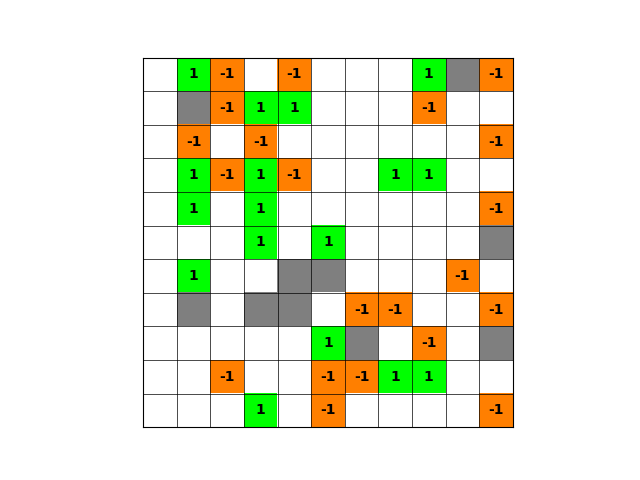
\includegraphics[width=60mm]{../results/maze_size_13/env.png}
        \caption{Maze size 13}
        \label{fig:random_env_4}
    \end{subfigure}
\end{figure}
\begin{figure}[H]
    \begin{subfigure}{.5\textwidth}
        \centering
        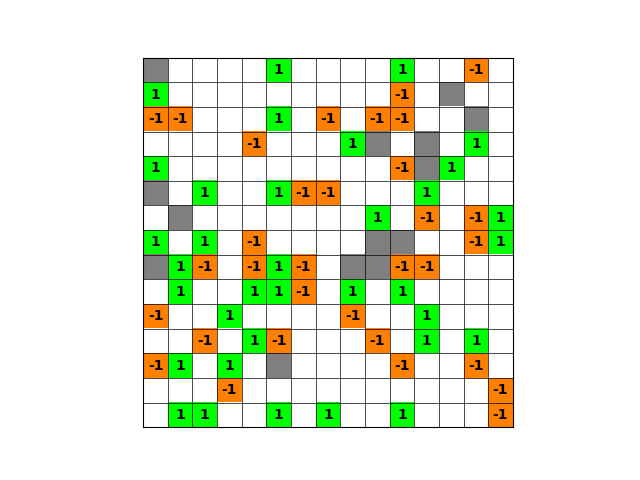
\includegraphics[width=60mm]{../results/maze_size_15/env.png}
        \caption{Maze size 15}
        \label{fig:random_env_5}
    \end{subfigure}
    \begin{subfigure}{.5\textwidth}
        \centering
        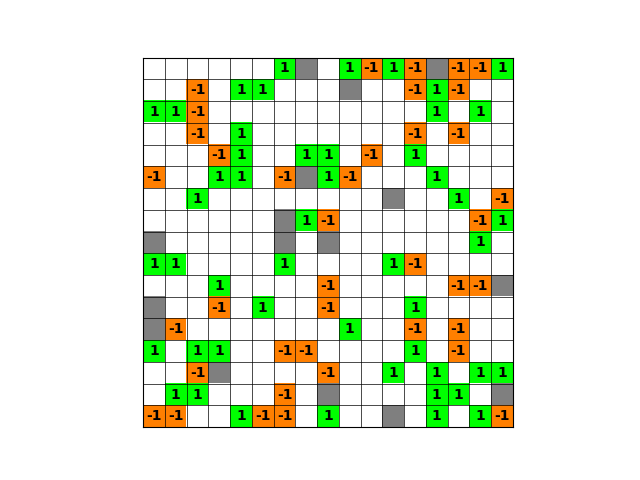
\includegraphics[width=60mm]{../results/maze_size_17/env.png}
        \caption{Maze size 17}
        \label{fig:random_env_6}
    \end{subfigure}
    \caption{Randomly generated environments.}
\end{figure}

\subsection{Comparison of value iteration and policy iteration}

\paragraph{Convergence among different maze complexity:} The convergence of value iteration and policy iteration for different maze size is shown in Figure \ref{fig:value_iteration_convergence} and Figure \ref{fig:policy_iteration_convergence}.

\begin{figure}[H]
    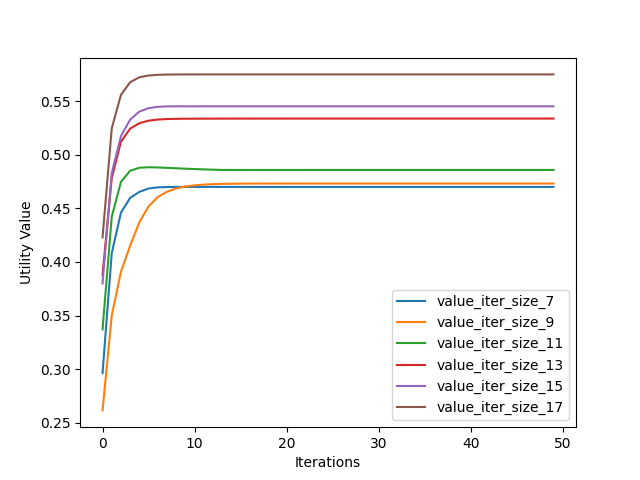
\includegraphics[width=100mm]{../results/value_iteration_curves.png}
    \caption{The value iteration curves for different maze size.}
    \label{fig:value_iteration_convergence}
\end{figure}

\begin{figure}[H]
    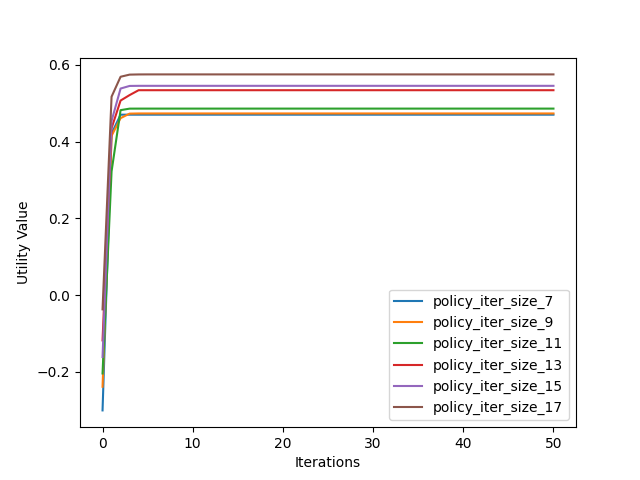
\includegraphics[width=100mm]{../results/policy_iteration_curves.png}
    \caption{The policy iteration curves for different maze size.}
    \label{fig:policy_iteration_convergence}
\end{figure}

This demonstrates that the complexity of the maze impacts the convergence of both value iteration and policy iteration. As the maze size increases, convergence becomes slower, and the final utility values tend to decrease.

\end{document}
